\section{Results}
\label{sec:results}


SHALL WE JUST ERASE "TARGET" OR "TARGETED" FROM TARGETED SAMPLING?

IN CASE WE WANT TO KEEP IT, SHOULDN'T IT BE "TARGETED"

This section presents the main results of the FRESNEL field campaign,
focusing on the integration of model forecasts, target sampling, and
data assimilation using autonomous underwater vehicles (AUVs). The
analysis combines CMS and statistical model forecasts (as described
in the Methods section) with in situ observations to assess how the
proposed data-cycle approach can enhance short-term ocean prediction
in a dynamic coastal environment.

Fig. \ref{fig:sst} provides an overview of the environmental conditions
observed during the three-day experimental window considered in this
study (29–31 October). The background fields correspond to the Level-3
Sea Surface Temperature (SST) product from Copernicus Marine Service
(\url{DOI:10.48670/moi-00310}). The operational area was relatively
compact, covering approximately 100 km² south of the Nazaré Canyon,
where the AUVs executed the planned target sampling missions. All
missions were planned using the target sampling algorithm to explore the
temperature variability predicted by the statistical model. On 31
October, however, XP2 performed a different mission, following a
cross-shore transect of approximately 13 km instead of a target-driven
pattern north of the canyon. This mission was designed to sample an
internal wave hotspot, but, for the purpose of this study, it serves as
an independent ground-truth dataset, collected in a distinct subregion
relative to where the data assimilation was applied. The XP2
observations are thus used as a reference for evaluating the forecast
cases (C–C4 and D–D4).

During this period, the coastal ocean was influenced by a late-season
upwelling–relaxation cycle. At the beginning of the sequence (29
October), the SST field reveals the characteristic signature of coastal
upwelling, with colder water masses extending offshore due to
wind-driven Ekman transport that brings subsurface, nutrient-rich waters
to the surface. In the following days (30–31 October), the weakening of
upwelling-favorable winds led to a relaxation phase, during which warmer
offshore waters gradually advanced toward the coast. This transition is
reflected in the SST maps by an overall warming trend in the nearshore
region, particularly evident on 1st October.

It is important to note that the SST imagery is partially affected by
cloud coverage, which limits the availability and accuracy of
satellite-derived temperature data. These gaps arise from the
radiometric constraints of indirect SST retrieval, resulting in reduced
spatial continuity and increased uncertainty near cloudy regions.
Despite these limitations, the SST patterns clearly capture the dominant
mesoscale features and coastal processes driving the observed
variability during the experiment.

These evolving conditions provided an ideal natural setting for testing
the adaptive sampling and data assimilation framework developed in
FRESNEL. The pronounced temperature gradients associated with the
upwelling front generated well-defined spatial and temporal variability,
allowing the evaluation of how AUV-based targeted observations can
improve the predictive skill of the statistical model in a real-world
coastal scenario.


\begin{figure}
  \centering 

  \subfigure[Sea surface temperature (SST) and XP2, XP3 and
  XP5 trajectories during the FRESNEL field campaign (29–31
  October) ADD new subfigure november.]
  {\label{fig:sst}\includegraphics[width=1\linewidth]{fig/Figure_sst_auv_l3_zoom.pdf}}

  \subfigure[Time–depth temperature evolution observed by XP2, XP3,
  and XP5 during the FRESNEL field campaign (29–31 October).]
  {\label{fig:temperatureprofiles}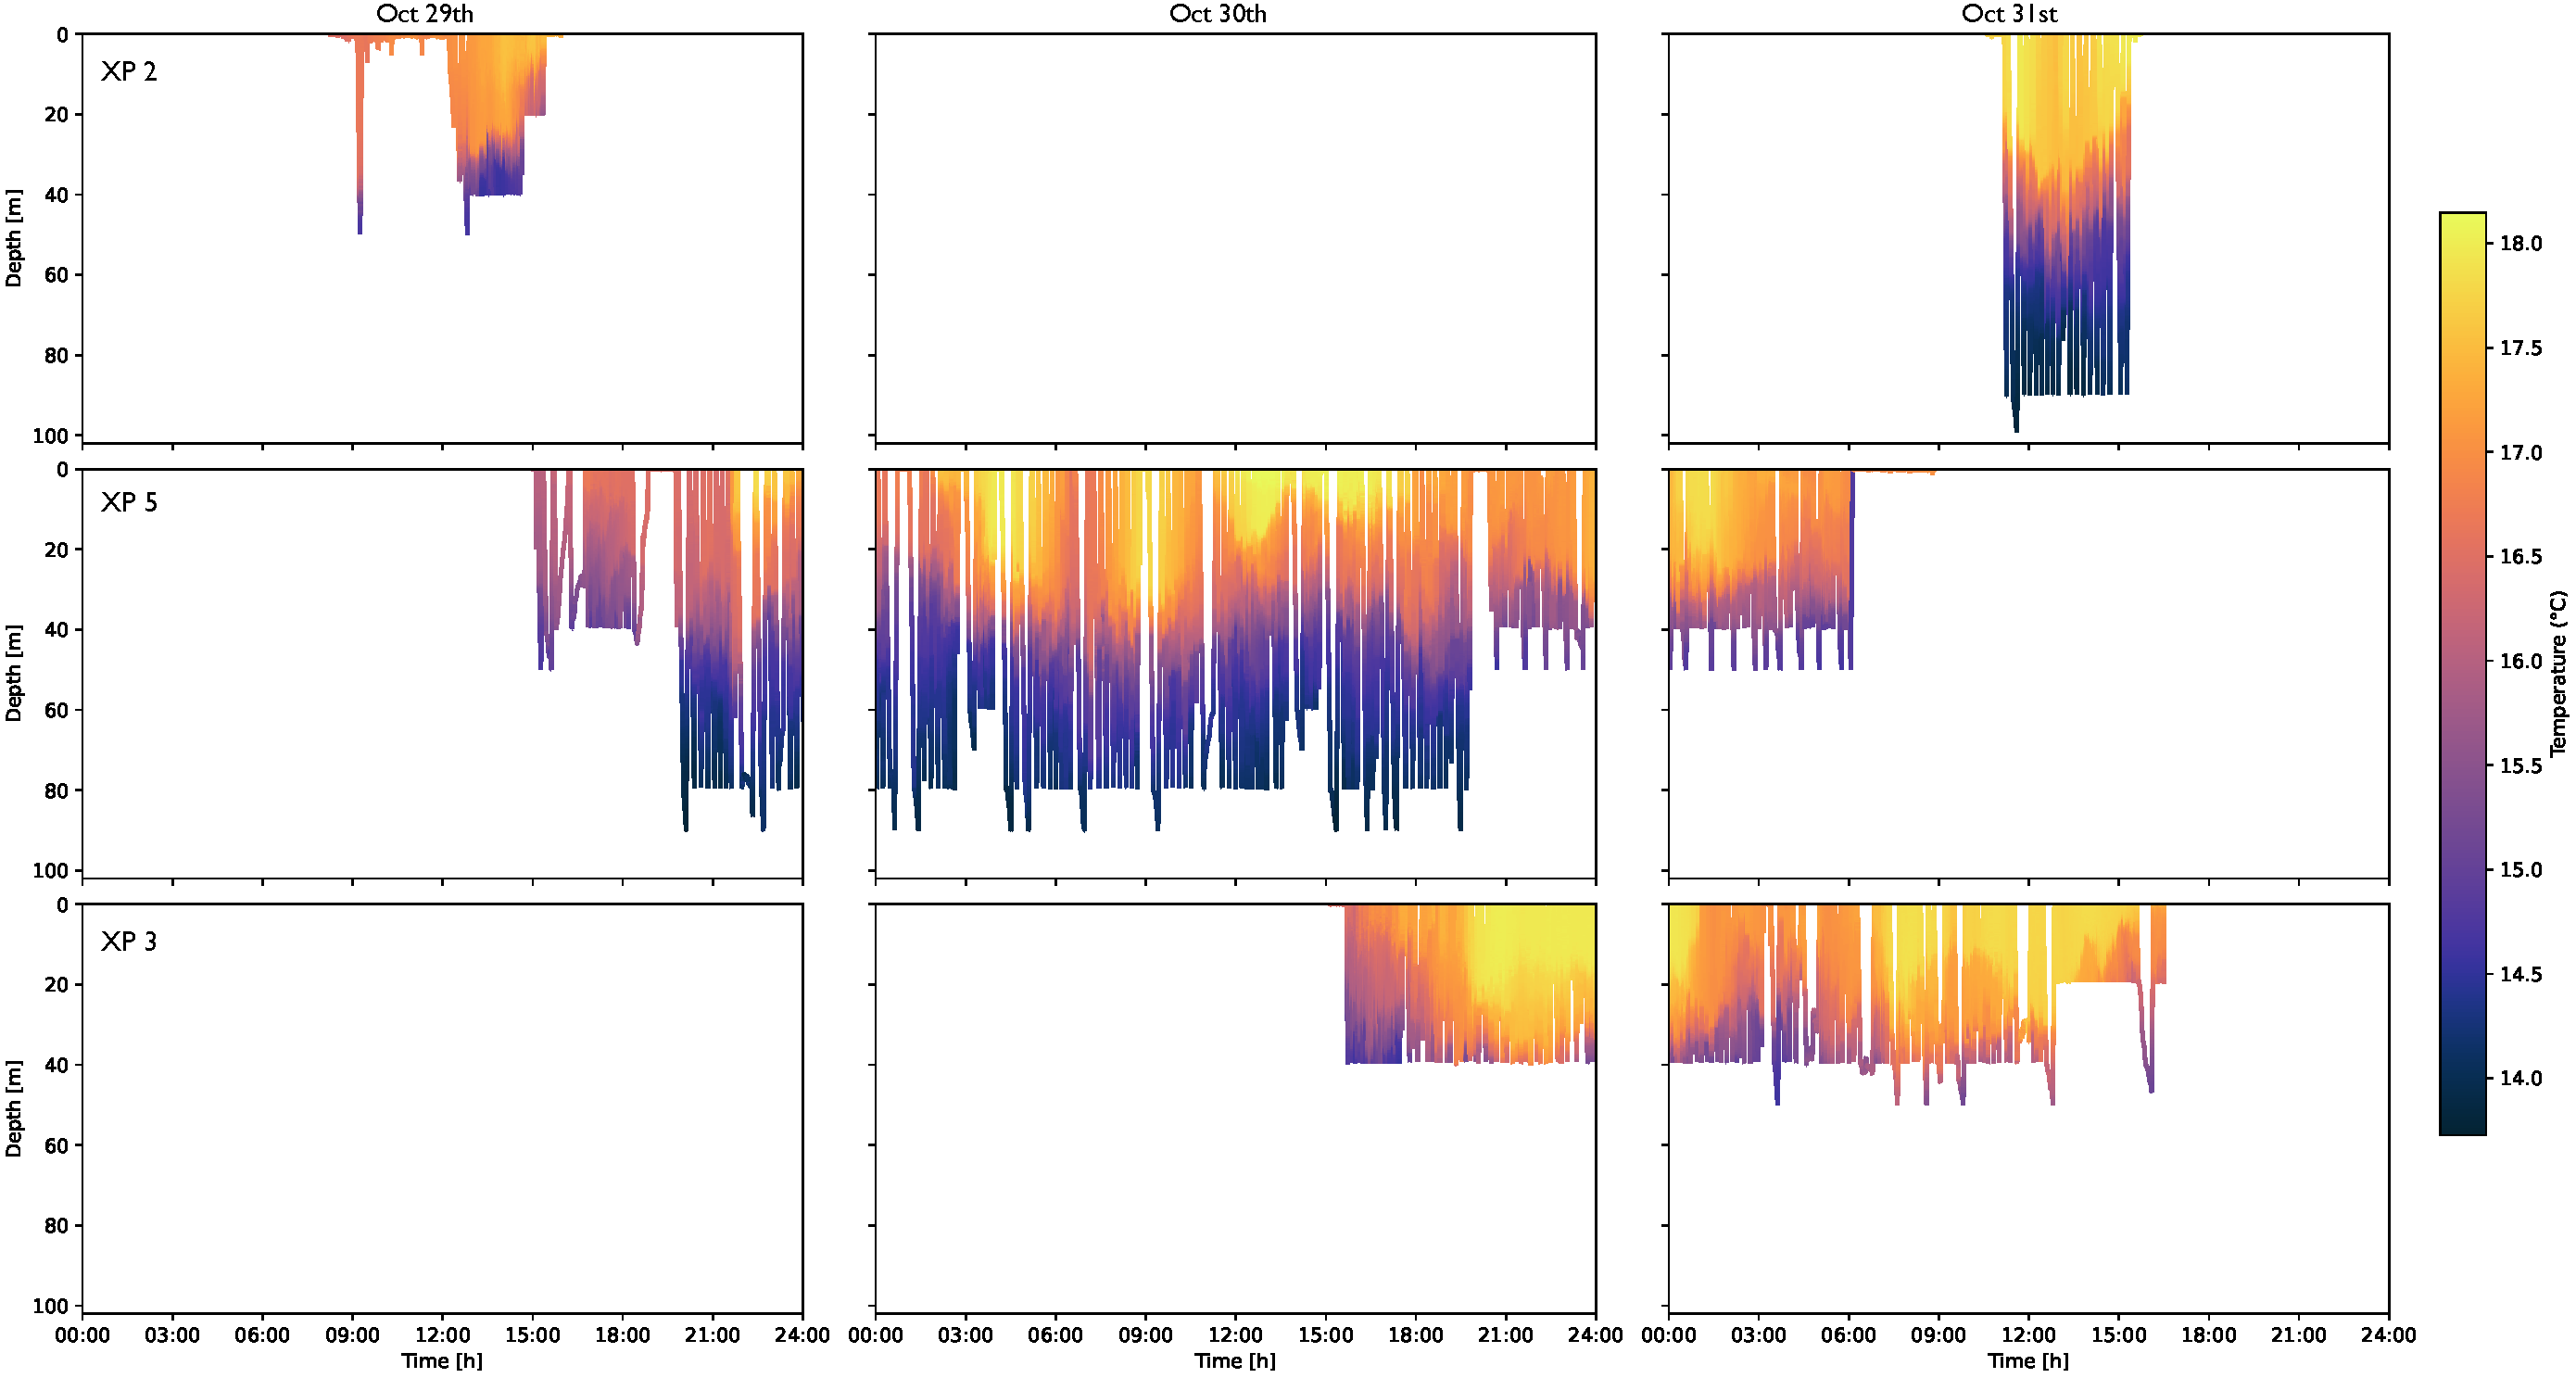
\includegraphics[width=1\linewidth]{fig/Figure2_100m.pdf}}

\end{figure}

Following the overview of the surface conditions,
Fig.\ref{fig:temperatureprofiles} presents the vertical temperature
distribution recorded by the LAUVs XP2, XP3, and XP5 during their
respective missions between 29 and 31 October. The panels show
temperature as a function of time and depth, illustrating the temporal
and vertical structure of the coastal water column throughout the
three-day experimental sequence.

XP2 operated on 29 October, XP5 on 29, 30, and 31 October, and XP3 on 30
and 31 October, with all vehicles capable of sampling the upper 100 m of
the water column. However, this depth range was not always achieved due
to logistical and bathymetric constraints. The temperature fields reveal
a thermocline and a progressive warming of the surface layer down to
approximately 40 m depth, with temperatures ranging from around 14 °C in
deeper layers to about 18 °C near the surface, reaching their maximum on
30 October afternoon during XP5’s mission.

It is important to note that the trajectories shown in the previous
figure might suggest that the AUVs remained continuously at sea for 24
hours each day. However, as Fig. \ref{fig:temperatureprofiles}
demonstrates, this was not the case. The vehicles can be deployed and
recovered multiple times per day, with operational windows limited by
logistics, weather, and available support assets. This figure,
therefore, also highlights the non-linear nature of field logistics in
multi-vehicle operations, where dynamic scheduling, resource allocation,
and environmental constraints determine the actual temporal coverage of
the missions.

The following section summarizes the quantitative evaluation of the
model’s predictive performance across all tested scenarios. Tables
\ref{table:Table_AB}, \ref{table:Table_C}, and \ref{table:Table_D}
present the RMSE between the statistical model forecasts and the in
situ temperature observations collected by the AUVs during the FRESNEL
campaign. These tables cover all experimental configurations examined
in this study, providing a comprehensive overview of how the
assimilation of targeted AUV data affects the model’s short-term
forecast accuracy and vertical consistency.


The first set of results, summarized in Table \ref{table:Table_AB},
corresponds to the initial phase of the FRESNEL experiments on days 29
and 30 October. Scenario A represents the baseline statiscal forecast
produced based CMS data. The B and B1 scenarios correspond to
forecasts for 30 October with and without the assimilation of
\textit{in situ} observations collected by XP2 during the previous
day, respectively.  Across the vertical profile, RMSE values in
scenario A range from approximately 0.48 $^{\circ}$C near the
surface to 1.33 $^{\circ}$C at 40 m, with a mean RMSE of about 0.74
 $^{\circ}$C. The errors increase with depth, indicating reduced
model skill in reproducing the subsurface thermal structure.  The
non-assimilated B scenario remains similar to A in the upper layers
but diverges below 20 m, confirming that the assimilation of recent
AUV data substantially improves the short-term forecast skill and
internal consistency of the model.  After assimilation, the B1 case
shows a consistent improvement throughout the column compared to the
non-assimilated B scenario, with RMSE values between 0.31 $^{\circ}$C and 0.55  $^{\circ}$C and an average of 0.39  $^{\circ}$C,
representing an overall reduction of nearly 50\% relative to B. This
improvement is most pronounced in the 5–20 m layer, coinciding with
the strongest vertical temperature gradients and the region most
densely sampled by the LAUVs.

\begin{figure}[!]
  \centering
1  \includegraphics[scale=0.7]{fig/rms_ABB1.png}
  \caption{RMSE (in  $^{\circ}$C) between statistical model forecasts and in situ LAUV temperature observations for 29–30
  October. Scenario A corresponds to the baseline statistical forecast generated based on CMS data up to 29 October. Scenarios B and B1
  represent forecasts for 30 October without and with the assimilation
  of LAUV observations collected by XP2, respectively. Values are
  shown for each depth level sampled during the missions.}
  \label{fig:rms_ABB1}
\end{figure}


The results for 31 October, summarized in Tables \ref{table:Table_C} and \ref{table:Table_D}, correspond to the most comprehensive phase of the experiment, in which multiple assimilation scenarios were tested. The C-series uses CMS data up to 30 October, whereas the D-series starts from CMS data up to 29 October, representing a less favorable statistical initial state. In both cases, the assimilation scenarios (C1–C4 and D1–D4) correspond to the incorporation of LAUVs temperature data collected during the previous days by XP2, XP3, and XP5.

A consistent reduction in statistical forecast error is observed across most vehicles and assimilation stages. In the C-series, the average RMSE across all LAUVs decreases from approximately 0.40 $^{\circ}$C in C to 0.31 $^{\circ}$C  in C4, while in the D-series, the mean RMSE drops from 0.55 $^{\circ}$C in D to 0.40 $^{\circ}$C  in D4. These improvements correspond to an average error reduction of 25–30\%, demonstrating that the assimilation of targeted observations can compensate for differences in the initial state and improve predictive accuracy.

It should be noted, however, that the improvement is not uniform across all vehicles. For XP3 and XP5, which performed target-sampling missions in the same area where previous assimilation data were collected, RMSE values show a clear reduction. In contrast, XP2, which on 31 October performed an independent cross-shore transect outside the main target region, exhibits a weaker response to assimilation. The implications of this behavior and its relevance for evaluating the predictive robustness of the framework will be further examined in the Discussion section.
Vertically, RMSE profiles show similar behavior in both experiment sets: errors tend to increase gradually below 25–30 m, where model uncertainty and unresolved variability are higher. However, this gradient weakens considerably in the fully assimilated cases (C4 and D4), particularly in the upper 30 m, where the assimilation of prior LAUV data significantly improves the representation of the temperature structure and short-term thermal evolution probably associated with the upwelling–relaxation transition.


\begin{figure}
  \centering 

  \subfigure[RMSE (in  $^{\circ}$C) between statistical model forecasts and in situ LAUV temperature observations for 29–30
  October. Scenario A corresponds to the baseline statistical forecast generated based on CMS data up to 29 October. Scenarios B and B1
  represent forecasts for 30 October without and with the assimilation
  of LAUV observations collected by XP2, respectively. Values are
  shown for each depth level sampled during the missions.]
  {\label{fig:sst}\includegraphics[width=1\linewidth]{fig/rms_bar_vechicle.png
  c}}

  \subfigure[Time–depth temperature evolution observed by XP2, XP3,
  and XP5 during the FRESNEL field campaign (29–31 October).]
  {\label{fig:temperatureprofiles}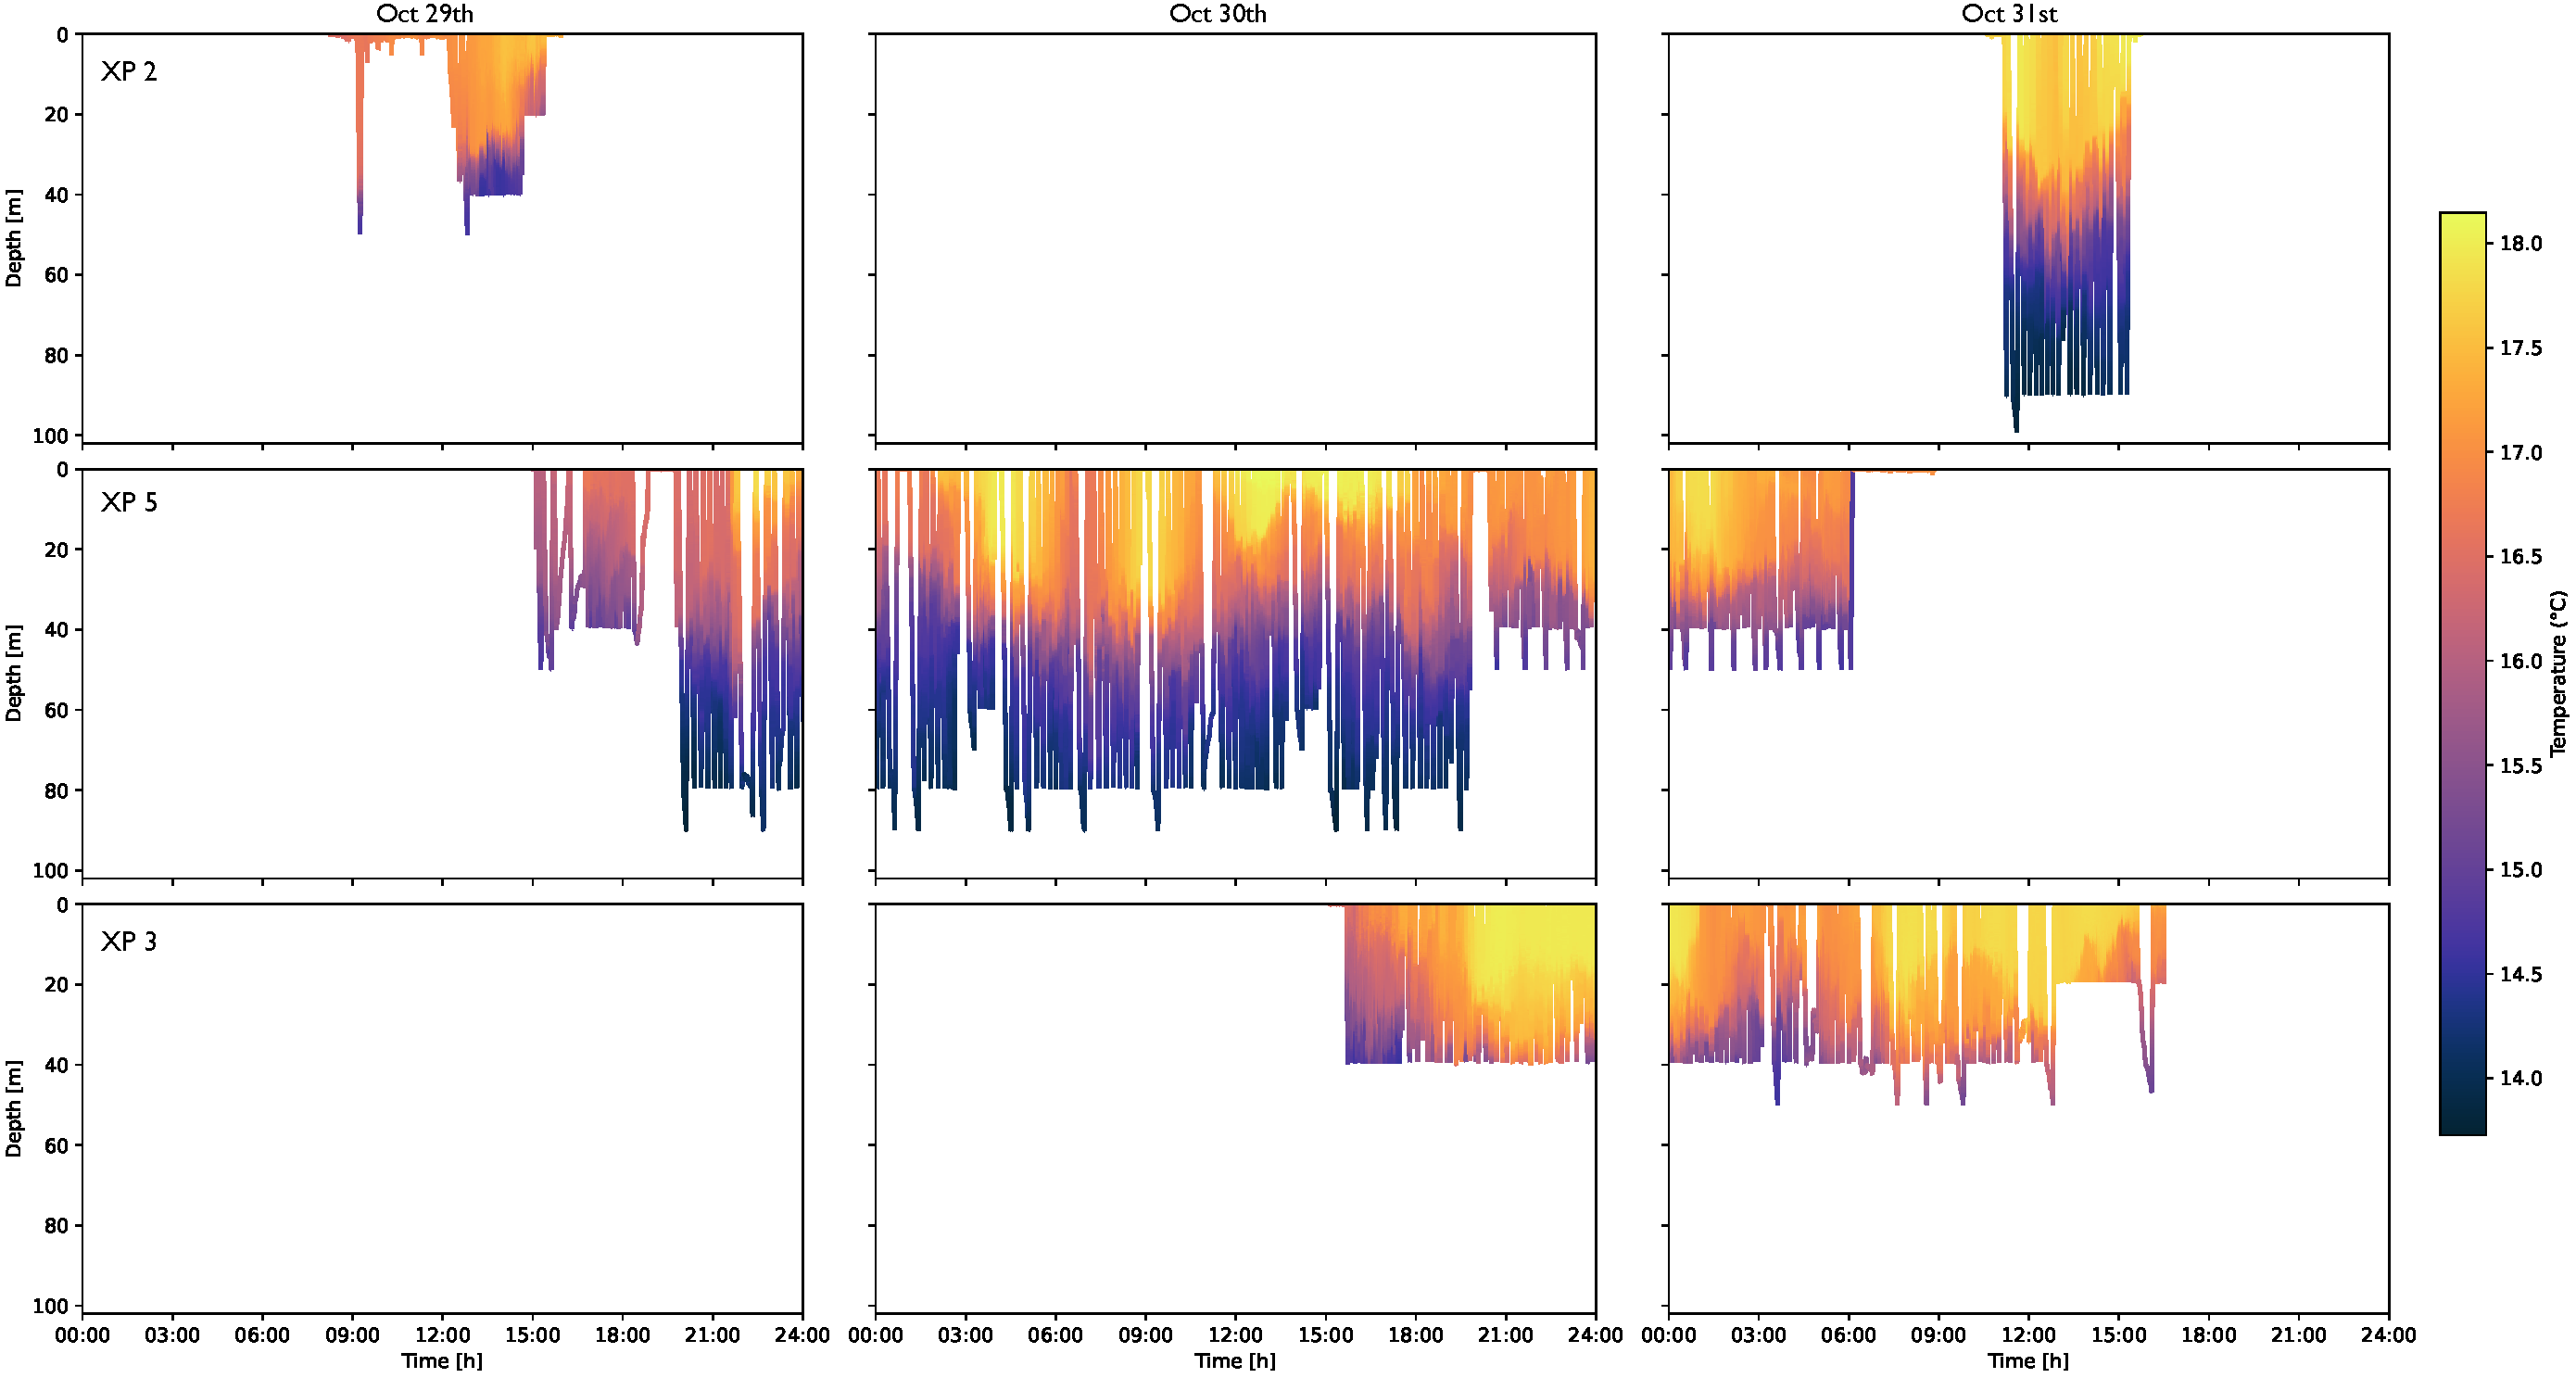
\includegraphics[width=1\linewidth]{fig/Figure2_100m.pdf}}

\end{figure}

\begin{figure}[!]
  \centering
  \sub
1  \includegraphics[scale=0.7]{fig/rms_ABB1.png}
  \caption{RMSE (in  $^{\circ}$C) between statistical model forecasts and in situ LAUV temperature observations for 29–30
  October. Scenario A corresponds to the baseline statistical forecast generated based on CMS data up to 29 October. Scenarios B and B1
  represent forecasts for 30 October without and with the assimilation
  of LAUV observations collected by XP2, respectively. Values are
  shown for each depth level sampled during the missions.}
  \label{fig:rms_c}
\end{figure}

\begin{figure}[!]
  \centering
1  \includegraphics[scale=0.7]{fig/rms_ABB1.png}
  \caption{RMSE (in  $^{\circ}$C) between statistical model forecasts and in situ LAUV temperature observations for 29–30
  October. Scenario A corresponds to the baseline statistical forecast generated based on CMS data up to 29 October. Scenarios B and B1
  represent forecasts for 30 October without and with the assimilation
  of LAUV observations collected by XP2, respectively. Values are
  shown for each depth level sampled during the missions.}
  \label{fig:rms_ABB1}
\end{figure}

To further interpret the RMSE results presented in the previous table,
Fig. \ref{fig:scatter} focuses on the most contrasted scenarios: the
baseline cases without assimilation (C and D) and those incorporating
the full set of AUV observations from previous days (C4 and D4). This
comparison highlights the point-wise behaviour of the statistical
model under minimum and maximum assimilation influence.

The four scatter plots compares the temperature values acquired in
situ by the AUVs on 31 October against the corresponding
geostatistical predictions derived from the statistical model under
each scenario. The observations include all available measurements
collected along the missions of XP2, XP3, and XP5 on that day (see
Fig. \ref{fig:sst} and \ref{fig:temperatureprofiles}. Colors indicate
the depth layers associated with the vertical discretization used in
the deterministic CMS model, which defines the vertical structure of
the statistical model.

In the baseline scenarios without assimilation (C and D), the scatter
plots exhibit a wide spread of points around the reference line,
indicating substantial discrepancies between the model predictions and
the observed AUV temperatures. These deviations are particularly
evident in ..., where surface temperatures tend to be
overestimated. This dispersion reflects the model’s limited ability to
accurately reproduce the vertical thermal structure when it relies
solely on CMS data without incorporating recent in situ information.

In contrast, the fully assimilated scenarios (C4 and D4) show a much
tighter clustering of points around reference, especially within the
upper layers, where the previous AUV missions had provided dense and
temporally relevant observations. This reduction in spread suggests a
clear improvement in predictive accuracy, indicating that the
assimilation of targeted measurements effectively constrains the
thermal structure and captures ongoing physical transitions in the
water column.



\begin{figure}[!]
  \centering
1  \includegraphics[scale=0.7]{fig/scatter.png}
  \caption{Comparison between in situ AUV observations (31 October)
    and geostatistical model predictions for scenarios C, C4, D, and
    D4. Shallower layers are shown in warmer colors (red to yellow),
    while deeper layers (>30 m) are progressively represented in
    cooler shades (green to blue). The dashed red line provides a
    reference for perfect agreement.  !not the final figure. need to
    correct and round values to 1 decimal place!}
  \label{fig:scatter}
\end{figure}


